\documentclass{./Paper}
\usepackage{graphicx}
\usepackage{subfigure}
\usepackage{float}
\title{现场教学}
\date{11月22日}
\begin{document}
\maketitle

本次现场教学,我们前往安吉古城遗址博物馆和安吉两弹一星事迹馆,开展了现场教学。在安吉古城遗址博物馆,我感受到八亩墩遗址的辉煌,透过历史遗迹和文物,领略了古代文明的智慧与创造力,这让我更加敬仰中华民族的悠久历史。

随后,我们来到两弹一星事迹馆,被展馆中的爱国精神深深触动。尤其是看到两弹一星功勋人物的手印时,我感到无比自豪和敬佩。他们中许多人与浙江大学有深厚渊源,作为浙大学子,我深感荣幸,也倍添责任感。他们用行动诠释了何为家国情怀,也激励着我为祖国的富强与发展不断努力。

此次活动中,我还报名成为小记者,为同学们拍摄活动照片,记录下珍贵瞬间。这次现场教学不仅让我感悟历史,厚植家国情怀,更坚定了为祖国奉献的决心。
\begin{figure}[H]
    \centering
    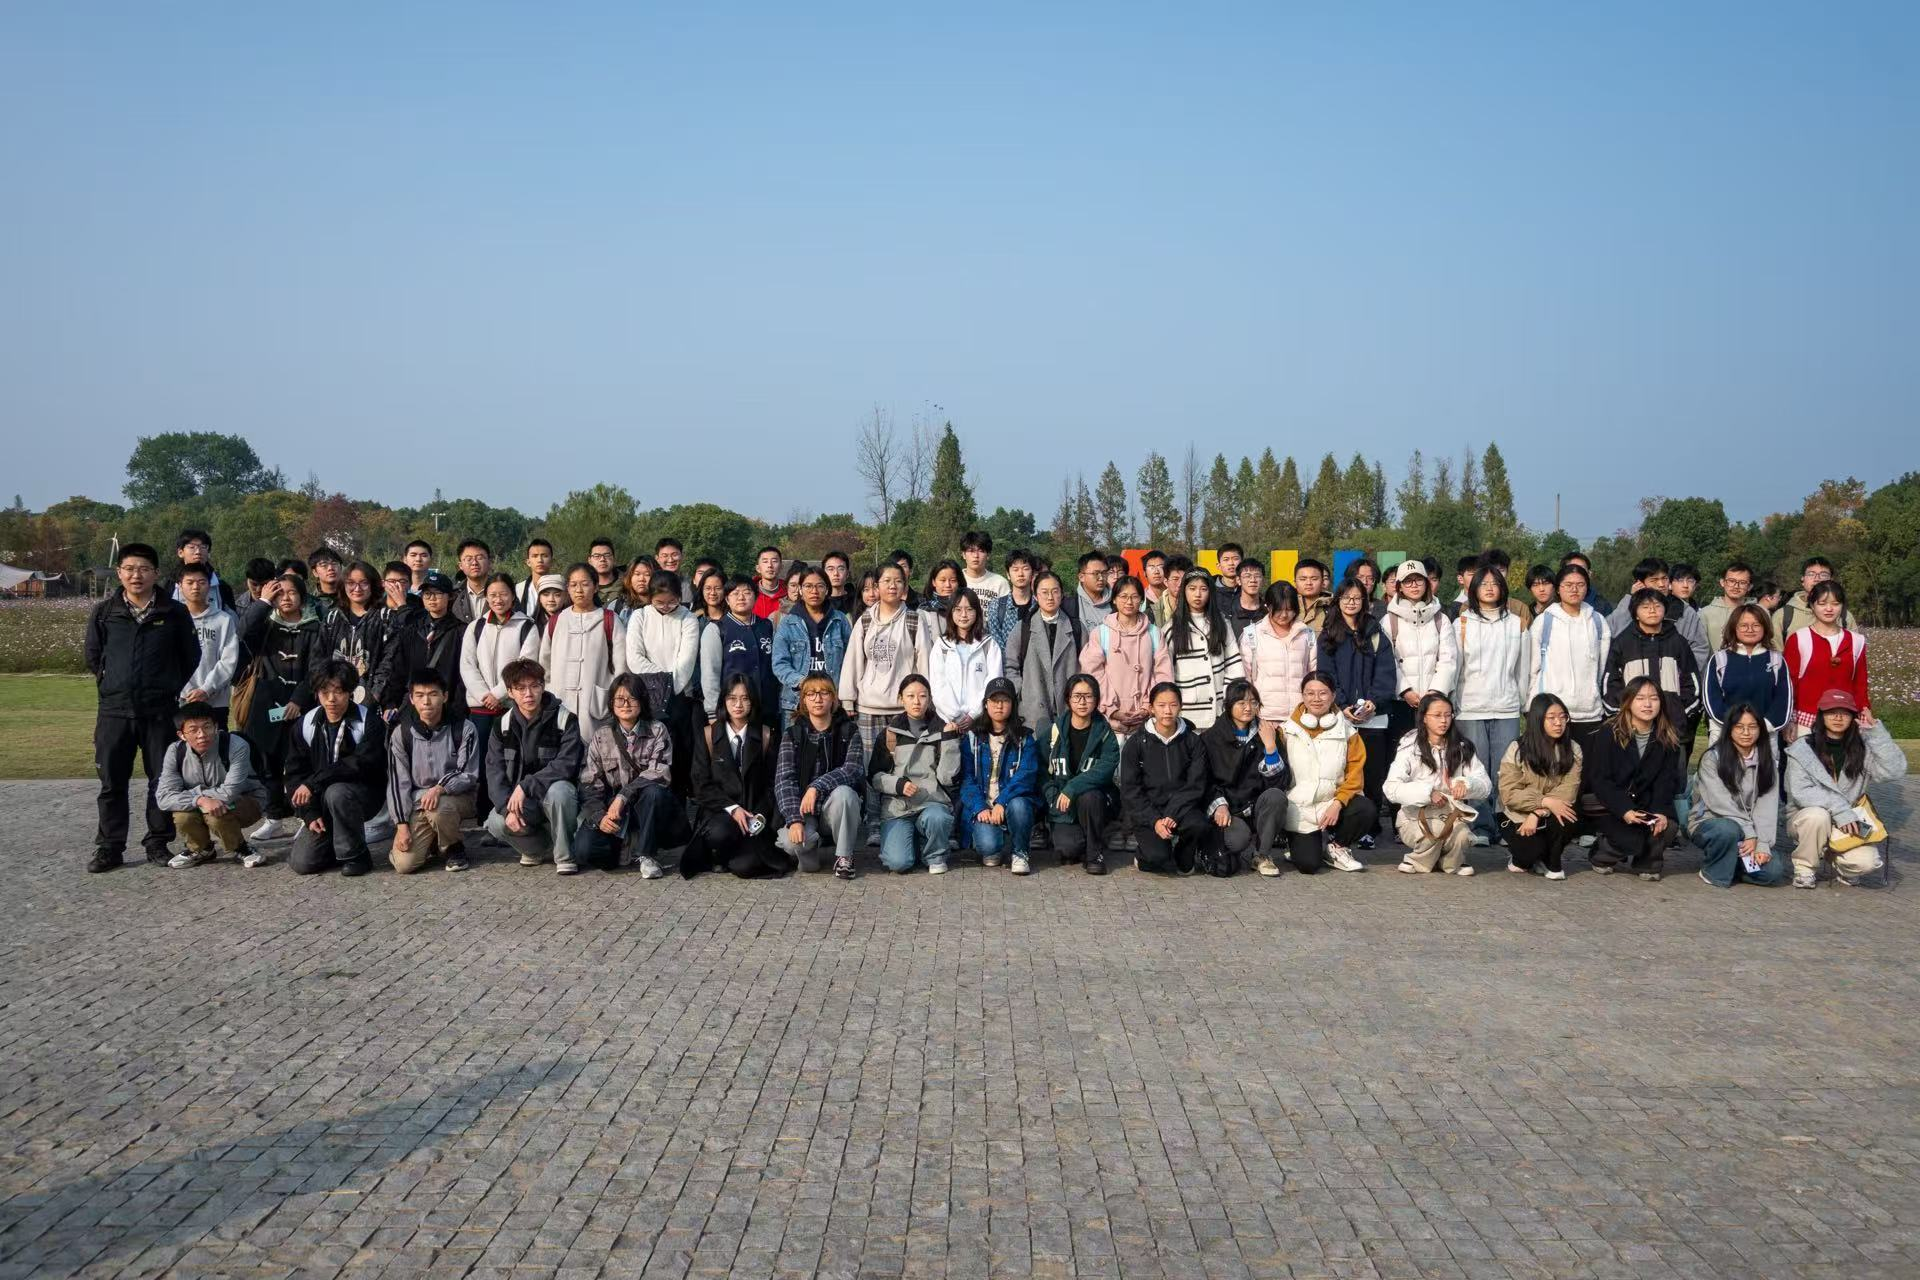
\includegraphics[width = .7\textwidth]{./pic/微信图片_20241224002224.jpg}
\end{figure}
\end{document}